\documentclass[a4paper]{report}

\usepackage[round]{natbib}
\usepackage[nottoc,numbib]{tocbibind}
\usepackage{graphicx}
\usepackage[noline,noend,algoruled]{algorithm2e}
\usepackage{amsmath}
\usepackage{amssymb}
\usepackage{amsthm}
\usepackage[small]{caption}
\usepackage{subcaption}
\usepackage[table]{xcolor}
\usepackage{hyperref}

\newtheorem*{definition}{Definition}
\defcitealias{intel12}{Intel\textsuperscript{\textregistered} 64 and IA-32
Architectures Optimization Reference Manual}

\begin{document}

\title{Automatic Structural Inference of Binary Protocols}
\author{Fredrik Appelros \and Carl Ekerot}
\date{\today}
\maketitle

\begin{abstract}
Communication protocols are the foundation of everyday networking tasks but
they are not always open in terms of available documentation. For reasons of
interoperability or the collection of statistics some protocols need to be
reverse engineered. This thesis presents a method based on density-based
clustering and byte distribution classification for automatically inferring the
structure of a protocol from a packet dump. We evaluate the precision of the
method for finding different packet types and for finding fields, both globally
across all packets and within the inferred packet types.
\end{abstract}

\tableofcontents

\chapter{Introduction}

\section{Background}
Communication protocols are the foundation of everyday networking tasks. Each
time a web page is served or an email is sent, a rigorous series of actions is
taken to ensure that the requested piece of information is relayed. The
information is packaged in a \emph{message} and both the syntax and the
semantics of these messages are defined by protocols.

Protocols may be open or closed in terms of available documentation. The reason
for them being closed might be that they are proprietary or simply because no
one invested in creating a documentation of the protocol in the first place.
Despite the lack of a documentation there still sometimes exists a need to
understand the inner workings of a certain protocol, e.g. when providing
interoperability between services. One infamous example of this is Microsoft's
proprietary SMB protocol which spawned the Samba project. This project was
created in an attempt to provide access to certain Windows services for
Unix-like operating systems. \citet{tridgell03} explains that the Samba project
reversed the SMB specification using techniques like \emph{fuzzing}, a process
where they inspect the response from a SMB server for a wide variety of
generated requests. Using this approach, it took many years until most of the
functionality of the SMB protocol had been implemented.

Another area where the need for inferring the structures of closed protocols is
in \emph{deep packet inspection} (DPI). Messages sent over a network are
usually constructed hierarchically. At the bottom there is only raw binary data
and at the top there is the application data, e.g. an email or a video. There
in between exists several layers that contain metadata which is used to make
sure that the data reaches its target and that it does not get corrupted during
transmission. As a message is sent from one party to another it traverses a
series of nodes in the network. These nodes only needs to look at the lower
parts of the hierarchical structure of the message in order to relay it. If a
node wants to conduct DPI however, the higher levels of the hierarchy is looked
at as well. To be able to do this the structure of the protocol needs to be
known.

There are many different reasons why one would want to perform DPI, one of
which is to provide \emph{quality of service} (QoS). QoS is needed in order to
gather statistics for Internet service providers that manage the networks. One
company that delivers QoS solutions is Procera Networks on whose behalf we are
writing this thesis.

In this thesis we have focused on finding the structure of binary protocols as
opposed to textual ones. The reason for this being that textual protocols are
intrinsically simple to read and understand and therefore do not require
advanced methods of analysis. Some of the methods described here are however
also applicable to textual protocols.

\section{Related work}
A popular approach to the problem of automatic inference of network protocols
has been to draw a parallel to bioinformatics. Byte-streams have been
processed using the same methodology as DNA sequence analysis in order
to mine patterns in protocol messages. \citep{beddoe05} explores the
possibilities of using bioinformatics methods such as multiple sequence
alignment in order to find patterns in both textual and binary protocols. These
principles have been applied in e.g. Netzob\footnote{http://www.netzob.org}, a
tool for protocol analysis.

Using techniques from bioinformatics in protocol analysis seems natural since
the analysis of messages, which may be viewed as the analysis of byte-streams,
is easily converted to the problem of sequence analysis. Methods such as
multiple sequence alignment does provide an insight to the structure of
protocols, but further analysis is needed in order to find semantic meaning in
segments of bytes.

Discoverer by \citeauthor{cui07} is an approach which is specifically modeled
after the behavior of network protocols. Discoverer tokenizes
network dumps into textual and binary tokens. From the tokens Discoverer
attempts to group messages based on their true message type, such as requests
or responses. After the grouping of messages, Discoverer seeks semantic meaning
in the tokens in common for each group of messages, and classifies the tokens
into a set of predefined classes. 

\citet{caballero12} proposes a method where protocol specifications are
constructed by monitoring the execution state of the client or server software
which utilizes the protocol. This approach has the obvious benefit of mapping
data stored in memory at one state to the data subsequently present in a
protocol message. This requires access to the actual software which generates
the messages. In many cases this may limit the analysis to the messages sent by
the client. When the server software is unavailable for execution state
monitoring, one must resort to other methods in order to further analyze the
protocol.

\chapter{Theory}

\section{Features}
In machine learning, a feature is a measurable property of the input data. An
example of a feature when working with images could be the intensity of light
for a certain pixel. Features do not need to directly correspond to a
physically measurable property however, instead they can be constructed by
transforming other features. These new high-level features can then be used
just like any other feature in order to simplify a complex problem.

One common type of complex problem is working with high dimensional data. There
are different ways to deal with such data; one of them being to use a solving
method that scales linearly. Another way is to reduce the dimensionality of the
problem itself.

\subsection{Principal component analysis}
\label{sec:pca}
One method to reduce the dimensionality of a problem is to use principal
component analysis (PCA). PCA is defined by \citet{jolliffe86} and transforms
the input data into another dataset where each dimension accounts for as much
variance as possible while requiring it to maintain orthogonality to the other
dimensions. The new dataset can be constructed to contain fewer dimensions than
the original data and will then capture as much variance as possible in the
given number of dimensions. PCA can be accomplished through singular value
decomposition of a matrix.

\section{Simple linear regression}
In statistics, a response variable $Y_i$ that is linearly dependent on an
explanatory variable $X_i$ can be modeled with a simple linear regression
model. The relationship between the two variables are then

\begin{equation}
    Y_i = \alpha + \beta X_i + \varepsilon_i
    \label{eq:slr}
\end{equation}

where $\alpha$ and $\beta$ are the \emph{regression coefficients} and
$\varepsilon_i$ is the error term. Given a set of data
$\displaystyle \{Y_i, X_i\}_1^n$ the regression coefficients can be estimated
through linear regression. This process is often called fitting as it can be
seen as trying to find the model with the best fit for the data. There are
different methods to do this as there is no consistent measure for what is the
best fit.

\subsection{Ordinary least squares}
Ordinary least squares (OLS) is a method for estimating the regression
coefficients in equation~\ref{eq:slr}. It does this by minimizing the sum of
squared residuals of the simple linear regression model. This can be formulated
as minimizing the following cost function.

\begin{equation}
    C(\alpha, \beta) = \sum_{i=1}^n(Y_i - \alpha - \beta X_i)^2
\end{equation}

The result of this is a model that minimizes the residuals globally across all
samples. This intrinsically makes the method \emph{non-robust}, i.e. sensitive
to outliers.

{
    \fontsize{10}{12}
    \selectfont
    \begin{algorithm}[t]
        \DontPrintSemicolon
        \BlankLine
        \KwIn{$D$, $M$, $n$, $\delta$, $\gamma$, $k$}
        \KwOut{$P_b$}
        \BlankLine
        $P_b \gets \varnothing$\;
        $\varepsilon_b \gets \infty$\;
        \For{$k$}{
            $I \gets n$ number of randomly chosen samples\;
            fit $M$ to $I$\;
            $I_m \gets$ samples where distance from $M \leq \delta$\;
            $I \gets I \cup I_m$\;
            \If{$|I| \geq \gamma$}{
                fit $M$ to $I$\;
                $\varepsilon \gets$ deviation from $M$ for all $I$\;
                \If{$\varepsilon < \varepsilon_b$}{
                    $P_b \gets$ parameters in $M$\;
                    $\varepsilon_b \gets \varepsilon$\;
                }
            }
        }
        \Return{$P_b$}
        \BlankLine
        \caption{RANSAC}
        \label{alg:ransac}
    \end{algorithm}
}

\subsection{RANSAC}
\label{sec:ransac}
Random Sample Consensus (RANSAC) \citep{fischler81} is a \emph{robust} method
for fitting a dataset to a model and was originally intended for image
analysis. The robustness of the method allows it to avoid the influence of
outliers in the model. Given a dataset $D$, a model $M$, a set of inliers $I$
and two confidence parameters, $\delta$ and $\gamma$, it works the following
way:

\begin{enumerate}
    \item Fit $M$ to $I$
    \item Find the samples that are within $\delta$ distance from $M$ and add
        those samples to $I$
    \item Continue if $|I|$ is at least $\gamma$
    \item Fit $M$ to $I$
    \item Evaluate $M$ from the residual of $I$
\end{enumerate}

One problem with this approach is that an initial set of inliers is required.
In most cases this is not available so we need to guess which samples might be
inliers. A simple solution to this is to take $n$ random samples and assume
that they are inliers. This only works if the assumption is actually true and
thus the resulting algorithm will be \emph{non-deterministic}, meaning that it
only produces a good fit with a certain probability. The algorithm is normally
run $k$ number of iterations until the probability of success is sufficiently
large. Pseudocode for RANSAC can be seen in algorithm~\ref{alg:ransac}.

The model that RANSAC operates on can be any kind of mathematical model, 
therefore when handling two-dimensional linear data the simple linear
regression model given in equation~\ref{eq:slr} can be used. This gives us a
method that solves the problem of simple linear regression but that is also
insensitive to outliers. A comparison between OLS and RANSAC on a dataset where
some samples have been replaced by random noise can be seen in
figure~\ref{fig:ransac}.

\begin{figure}[t]
    \centering
    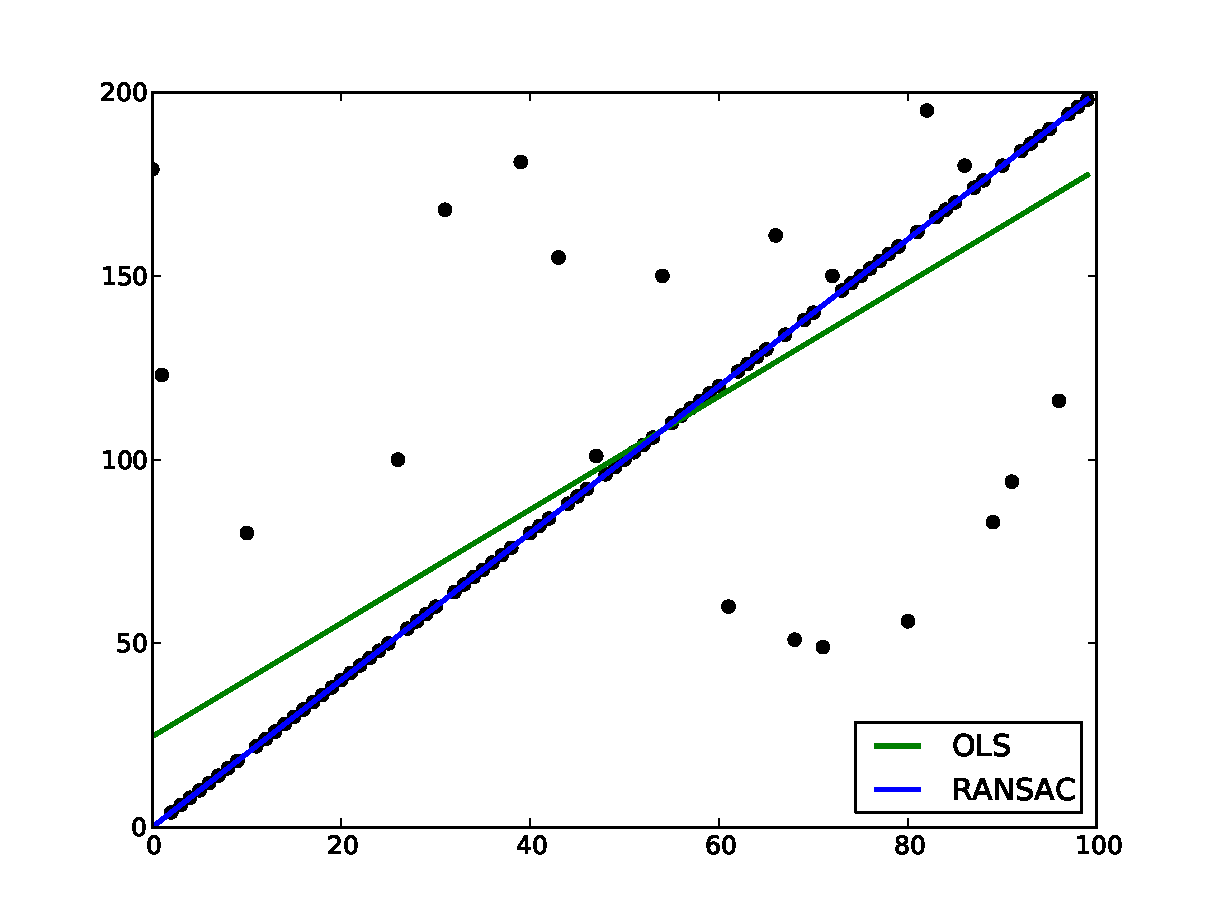
\includegraphics[width=0.8\textwidth]{ransac}
    \captionsetup{width=0.8\textwidth}
    \caption{A comparison between OLS and RANSAC on a dataset containing
    outliers.}
    \label{fig:ransac}
\end{figure}

\section{Clustering}
A clustering is a grouping of samples based on similarity with respect to their
features. The features are predefined to represent distinct properties of the
samples. Similarities between samples are normally represented as distances in
an $n$-dimensional space, where $n$ is the number of features. Distances may be
calculated using any suitable norm.

In cluster analysis, the goal is normally to find a clustering from a
set of samples such that the membership of a cluster represents some true
relationship. In some clustering algorithms such as K-means \citep{macqueen67},
the number of clusters are predefined. When the number of clusters are unknown,
other algorithms such as DBSCAN, OPTICS and hierarchical clustering methods may
be used.

The clustering algorithm we use in our method is OPTICS, which is based on
DBSCAN. In the rest of this section we will explain these algorithms and
provide examples based on protocol data.

\subsection{DBSCAN}
DBSCAN is a \emph{density-based} clustering algorithm, as opposed to
partitioning clustering algorithms such as K-means. Density-based clustering 
algorithms provides the benefit of not having to provide an estimated number 
of clusters as a parameter to the algorithm.

DBSCAN was first presented by \citet{ester96}. The algorithm takes a set of 
samples $D$ and two parameters, $MinPts$ and $\varepsilon$. $MinPts$ decides
how many samples that are needed in order to form a cluster.

The densities are defined by the distances between a set of points.
The algorithm introduces the definition \emph{$\varepsilon$-neighborhood}
$N_{\varepsilon}(p)$ for a point $p$. The samples which are in 
$N_{\varepsilon}(p)$ are given by the following condition:

\begin{equation}
    N_{\varepsilon}(p) = \{ q \in D ~|~ dist(p,q) < \varepsilon  \}
    \label{eq:eps}
\end{equation}

The samples in $N_{\varepsilon}(p)$ are defined as
\emph{directly density-reachable} from $p$. Given that
$|N_{\varepsilon}(p)| \ge MinPts$, the samples in $N_{\varepsilon}(p)$ forms a
cluster, and $p$ is a \emph{core point}.

A cluster is not limited to containing samples which are directly
density-reachable. The DBSCAN algorithm also defines that samples which are
not directly density-reachable may be \emph{density-reachable}.
A sample $q$ is density-reachable from a sample $p$ if there is a set of samples
$S = \{s_1, .., s_n\}$ where $p = s_1$, $q = s_n$ and $s_{i+1}$ is directly
density-reachable from $s_i$ for $0 < i < n$.

Since the density-reachable relationship is not symmetric, a looser
relationship is introduced: \emph{density-connected}. Two samples $p$ and
$q$ are density-connected if there exists a third point $o$ from which both
$p$ and $q$ are density-reachable. The density-connected relationship
is symmetric.

With these relationships, the algorithm defines cluster membership as
follows:

\begin{definition}
    The following conditions needs to be satisfied for a point $q$ to be a
    member of a cluster $C$, given that there is a sample $p \in C$:
    \begin{enumerate}
        \item $q$ is density-reachable from $p$
        \item $q$ is density-connected to $p$
    \end{enumerate}
\end{definition}

One of the drawbacks of DBSCAN is that it can only find clusters with a density
higher than the density decided by the $\varepsilon$-parameter. It is also hard
to estimate the $\varepsilon$ and $MinPts$-parameters for an unknown dataset.
This makes DBSCAN suitable for classifying data into known classes, but not as
suitable for finding underlying structures in entirely unknown datasets. In
figure~\ref{fig:dbscan} is an example of DBSCAN running on 5000 packets of DNS
data. The parameters are manually selected to $\varepsilon = 0.085$ and
$MinPts = 200$.

\begin{figure}[h]
    \centering
    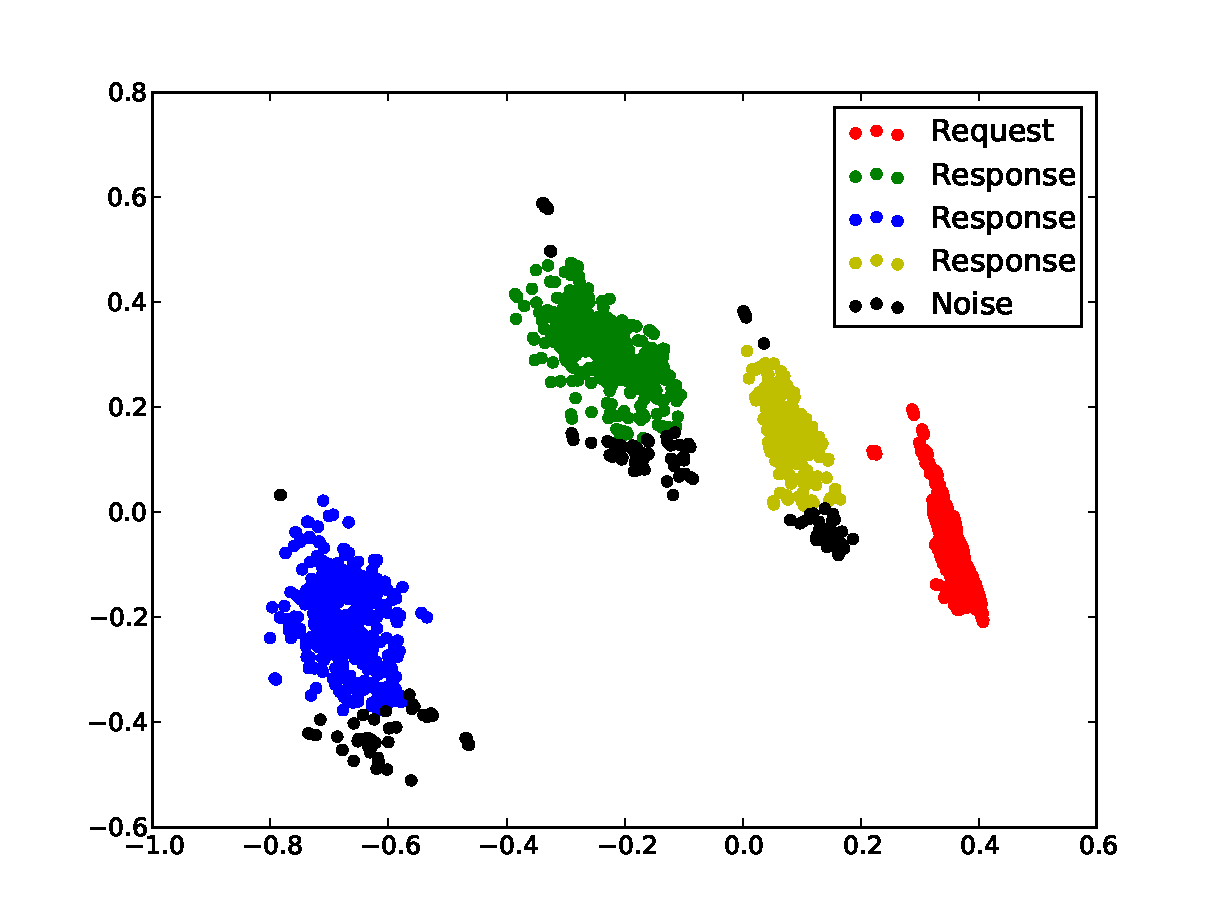
\includegraphics[width=0.8\textwidth]{dbscan_dns}
    \captionsetup{width=0.8\textwidth}
    \caption{An example of clustering with DBSCAN running on samples generated
    from 5000 packets of DNS data. The samples has been projected down to two
    dimensions using PCA (see section~\ref{sec:pca}).}
    \label{fig:dbscan}
\end{figure}

\subsection{OPTICS}
Addressing the difficulties in selecting parameters for DBSCAN,
\citet{ankerst99} introduced the OPTICS algorithm, which is an extension of
the concepts introduced in DBSCAN. OPTICS uses the definitions
\emph{directly density-reachable}, \emph{density-reachable} and
\emph{density-connected} which were described in the DBSCAN algorithm, but
eliminates the need for an explicit $\varepsilon$ parameter. Instead the
$\varepsilon$ parameter is interpreted as the largest distance to consider
when clustering. The results is an algorithm which is less sensitive to
user-specified parameters, and is able to find clusters with varying densities.

One important aspect of OPTICS is that it does not generate actual clusters.
Instead, it generates an \emph{ordering} of samples and a set of corresponding
\emph{reachability-distances} which reveals density-based structure in the
input data. The OPTICS algorithm extends DBSCAN with the definitions
\emph{core-distance} and \emph{reachability-distance}.
\\[0.5cm]
Core-distance is a measurement of the distance $\varepsilon$ which is required
for a sample $p$ to be a core point. That is, a core distance is the distance
$\varepsilon$ which satisfies $|N_{\varepsilon}(p)| = MinPts$.

\begin{definition}
    The core-distance for a sample $p$ is defined as:
\[
    \begin{cases}
        \text{UNDEFINED}, & \text{if $|N_{\varepsilon}(p)| < MinPts$}\\
        \text{Min $\varepsilon$ which satisfies  $|N_{\varepsilon}(p)| =
        MinPts$}(p), & \text{otherwise}
    \end{cases}
\]
\end{definition}

The core-distance is $UNDEFINED$ when an upper limit on $\varepsilon$ is
given as a parameter to the algorithm. This parameter is not required,
although it has an impact on the runtime of the algorithm.
\\[0.5cm]
The reachability-distance of a sample $p$ is the smallest distance which is
needed for $p$ to be directly density-reachable to a core point $q$ for some
$\varepsilon$. 

\begin{definition}
    The reachability-distance of a sample $p$ with respect to some sample $q$
    is defined as:
\[
    \begin{cases}
        \text{UNDEFINED}, & \text{if $|N_{\varepsilon}(q)| < MinPts$}\\
        \text{max(core-distance($q$), distance($q$, $p$))}, & \text{otherwise}
    \end{cases}
\]
    where distance($q$, $p$) is the smallest $\varepsilon$ for which $q$ is
    density-reachable from $p$.
\end{definition}

From the ordering and reachability-distances, the cluster structure may be
visualized in a \emph{reachability-plot}. The reachability-plot provides an
overview of the output from OPTICS as a bar-plot where the bars represent
reachability-distances in the ordering generated by OPTICS.

An example of a reachability plot generated from 5000 DHCP-packets with 
$MinPts = 500$ is shown in figure~\ref{fig:rplot}. Valleys in the
reachability-plot represents samples which are close to each other. Spikes
represents a large difference in distance between the samples to the left and
right of the spike.

The pseudocode algorithm is given in algorithm~\ref{alg:optics}.

\begin{figure}[t]
    \centering
    \begin{subfigure}[b]{0.48\textwidth}
        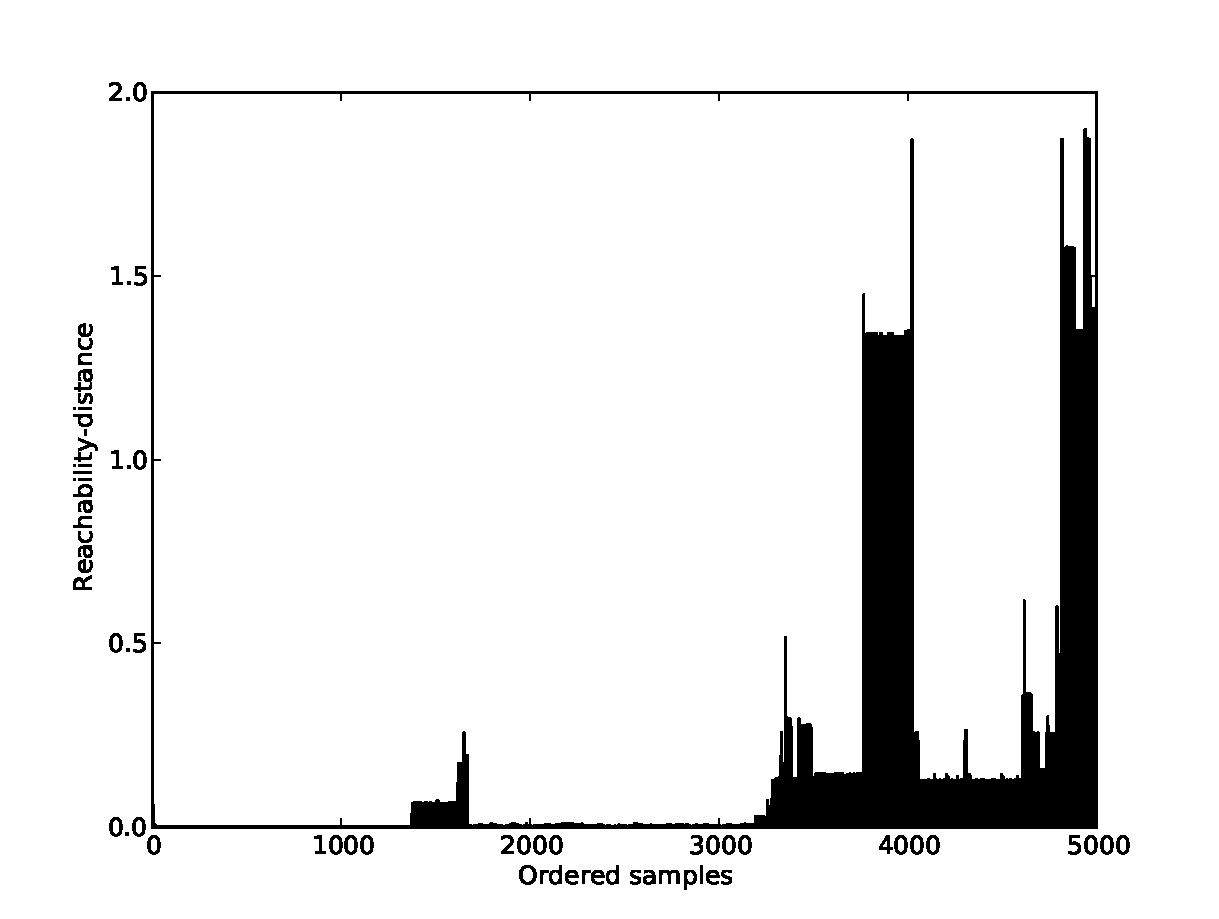
\includegraphics[width=\textwidth]{rplot_dhcp}
        \caption{Reachability-plot for 5000 DHCP-packets with $MinPts = 200$.}
        \label{fig:rplot}
    \end{subfigure}
    \quad
    \begin{subfigure}[b]{0.48\textwidth}
        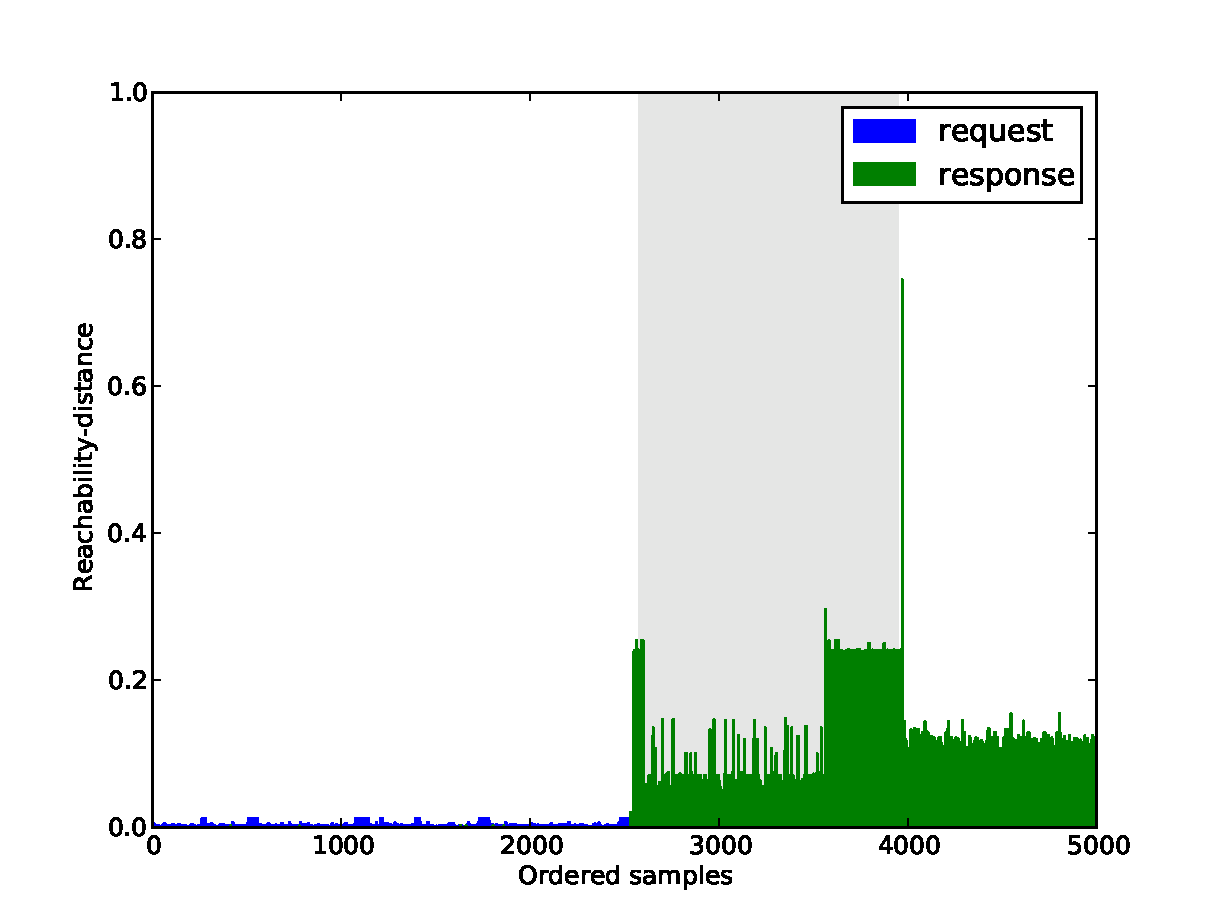
\includegraphics[width=\textwidth]{hierextr}
        \caption{Hierarchical extraction for 5000 DNS-packets with
        $MinPts = 200$.}
        \label{fig:hierextr}
    \end{subfigure}
    \caption{Reachability-plots generated from the ordering and
    reachability-distances given by OPTICS.}
    \label{fig:rplots}
\end{figure}

{
    \fontsize{10}{12}
    \selectfont
    \begin{algorithm}[H]
        \DontPrintSemicolon
        \BlankLine
        \KwIn{$D$, $MinPts$, $\varepsilon$}
        \KwOut{$ordering$, $reachability$-$distances$}
        \BlankLine

        $reachability$-$distances \gets \varnothing$\;
        $ordering \gets \varnothing$\;
        $seeds \gets 0,1,...,|D|$\;
        $i \gets 0$\;

        \While{$|seeds| > 1$} {
            $p \gets seeds.get(i)$\;
            $seeds.remove(i)$\;
            $ordering.add(p)$\;

            \If{$core$-$distance_{\varepsilon, MinPts}(p) \le \varepsilon$}{
                $neighbors \gets N_{\varepsilon}(p)$\;
                \For{each neighbor sample $n$} {
                    $rdist \gets \text{$reachabilty$-
                        $distance_{\varepsilon, MinPts}$}(n,p)$\;
                    $reachability$-$distances[n] \gets rdist$\;
                }
                $i \gets$ seed with least reachability-distance\;
            }
            \Else{
                $i \gets seeds.first$\;
            }
        }
        \CommentSty{/* Process last remaining seed */}\;
        $ordering.add(seeds.first)$\;
        $reachability$-$distances[0] \gets 0$\;
        \Return{$ordering$, $reachability$-$distances$}
        \BlankLine
        \caption{OPTICS}
        \label{alg:optics}
    \end{algorithm}
}

\subsubsection{Cluster extraction}

\citeauthor{ankerst99} describes the principles of the OPTICS algorithm as
running DBSCAN for an infinite number of distance parameters $\varepsilon_i$
in the interval $0 \le \varepsilon_i \le \varepsilon$. They also explain that
extracting clusters from the OPTICS ordering and reachability-distances using
a static reachability-distance threshold $\varepsilon_i$ gives a clustering
which is roughly equivalent to the clustering obtained when running DBSCAN
with the same $MinPts$ and $\varepsilon = \varepsilon_i$.

\citet{sander03} describes a hierarchical cluster extraction algorithm for
OPTICS. As opposed to the DBSCAN-equivalent extraction approach, hierarchical
cluster extraction retains many of the properties which comes with OPTICS,
such as finding clusters with varying densities and subclusters nested in larger
clusters.

The algorithm takes an ordering and reachability-distances from OPTICS and
builds a hierarchical representation of the clustering in the form of a tree,
where the leaves are clusters.

The pseudocode for hierarchical extraction is given in 
algorithm~\ref{alg:hierextr}. Figure~\ref{fig:hierextr} is the result of
the algorithm running on the same DNS dataset as figure~\ref{fig:dbscan}
with $MinPts = 200$. The algorithm yields three clusters, each cluster
distinguished by changing background color. The true types \emph{request} and
\emph{response} are colored blue and green respectively in the reachability
plot. Note that the algorithm is rather insensitive to the $MinPts$-parameter,
and that the true types of DNS may be extended to different record types such
as A/AAAA/CNAME-records.

{
    \fontsize{10}{12}
    \selectfont
    \begin{algorithm}[t]
        \DontPrintSemicolon
        \BlankLine
        \SetKwBlock{Fn}{function}{end}
        \KwIn{$ordering$, $reachability$-$distances$}
        \KwOut{$clustering$}
        \BlankLine

        $R \gets reachability$-$distances$ arranged according to $ordering$\;
        $n \gets$ number of samples\;
        $L \gets$ indices of local maxima in $R$\;
        Sort $L$ on $R[L_i]$\;
        $R_{max} \gets$ $R[L.last]$\;
        $leaves \gets \varnothing$\;

        \Fn(\emph{cluster\_tree(node, parent, L)}:){
            \If{$L$ is empty}{
                $leaves.add(node)$\;
                \Return\;
            }
            $s \gets L.pop()$\;
            $node.split \gets s$\;
            $sign\_thres \gets significant$-$ratio * R[s]$\;
            Create two new nodes, $N1$ and $N2$\;
            $N1.samples \gets$ samples left of $s$\;
            $N2.samples \gets$ samples right of $s$\;
            $L1 \gets $ local maxima left of $s$\;
            $L2 \gets $ local maxima right of $s$\;
            \If{$N1$ and $N2$ has average reachability $<$ $sign\_thres$}{
                \If{$|N1| > MinPts$}{
                    $children.add(\{N1, L1\})$\;
                }
                \If{$|N2| > MinPts$}{
                    $children.add(\{N2, L2\})$\;
                }
                \If{$children$ is empty}{
                    $leaves.add(node)$\;
                    \Return\;
                }
                \If{$R[s] \approx R[parent.split]$}{
                    \For{$\{child, L\}$ in $children$}{
                        $parent.children.add(child)$\;
                    }
                    $parent.children.remove(node)$\;
                    $p \gets parent$\;
                }
                \Else{
                    \For{$\{child, L\}$ in $children$}{
                        $node.children.add(child)$\;
                    }
                    $p \gets node$\;
                }
                \For{$\{child, L\}$ in $children$}{
                    \emph{cluster\_tree(child, p, L)}\;
                }
            }
            \Else{
                \emph{cluster\_tree(node, parent, L)}\;
            }
        }
        \BlankLine
        Create node $root$ containing all samples\;
        \emph{cluster\_tree(root, null, L)}\;
        \BlankLine
        \caption{Hierarchical Cluster Extraction}
        \label{alg:hierextr}
    \end{algorithm}
}

\subsection{Clustering metrics}
When measuring the quality of a clustering from a clustering algorithm, a
number of metrics are defined. These metrics reflects the quality of the
features as well as the clustering algorithm. The metrics requires labels
given from the clustering algorithm as well as a \emph{truth}, i.e. the true
classes of the samples. The clustering metrics in this section are defined
by \citet{rosenberg07} using information entropy.

\subsubsection{Homogenity score}
Homogenity is satisfied when every cluster only contains members of a single
true class. When completely satisfied, $h = 1$. If every cluster contains
samples from different true classes then $h = 0$. When some clusters only
contains members from one true class while other contains mixed true classes
then $0 < h < 1$.

\subsubsection{Completeness score}
Completeness is satisfied when all members of a true class are in the same
cluster. When completely satisfied, $c = 1$. If all members of a true class
are spread out over different clusters then $c = 0$. When some true classes
are spread out while other are contained in single clusters then
$0 < c < 1$.

\subsubsection{V-Measure score}
V-Measure is a weighted harmonic mean of homogenity and completeness, and
is defined by \citeauthor{rosenberg07} as:

\[
    V_{\beta} = \frac{(1 + \beta) * h * c}{(\beta * h) + c}
\]

We weigh homogenity and completeness equally in our application, thus setting
$\beta = 1$.

\section{Sequence alignment}
The problem of aligning sequences with one another originally arose in the area
of bioinformatics. There, a need to find similarities in long chains of amino
acids existed. One of the first methods that solved this problem was the
Needleman-Wunsch algorithm \citep{needleman70}. The algorithm finds the maximal
number of matching symbols between two sequences, allowing for gaps to be
inserted into either sequence. This is done by tracing a path through an
alignment matrix where each element represents a possible matching of symbols
between the sequences.

Originally, the path was built only with respect to the number of matching
identical symbols and not to the number of mismatches or gaps. This has since
been improved upon to include pairwise scores for symbol matching and penalties
for gaps. The different scores used when matching symbols is typically given in
a similarity matrix. An example of such a matrix for a small alphabet of
symbols is seen in figure~\ref{fig:simmatrix}.

\begin{figure}[t]
    \centering
    \begin{subfigure}[b]{0.3\textwidth}
        \begin{tabular}{| c | c | c | c | c |}
            \hline
              &  A &  C & G &  T \\ \hline
            A &  2 &  1 & 0 &  1 \\ \hline
            C &  1 &  2 & 1 & -1 \\ \hline
            G &  0 &  1 & 2 &  1 \\ \hline
            T &  1 & -1 & 1 &  2 \\ \hline
        \end{tabular}
        \caption{The similarity matrix for the alphabet.}
        \label{fig:simmatrix}
    \end{subfigure}
    \quad
    \begin{subfigure}[b]{0.55\textwidth}
        \begin{tabular}{| c | c | c | c | c | c | c | c | c |}
            \hline
            & & A & T & T & C & G & C & T \\ \hline
            &\cellcolor[gray]{0.9}0 & -1 & -2 & -3 & -4 & -5 & -6 & -7 \\
            \hline
            A & -1 &\cellcolor[gray]{0.9}2 & 1 & 0 & -1 & -2 & -3 & -4 \\
            \hline
            C & -2 &\cellcolor[gray]{0.9}1 & 1 & 0 & 2 & 1 & 0 & -1 \\ \hline
            T & -3 & 0 &\cellcolor[gray]{0.9}3 & 3 & 2 & 3 & 2 & 2 \\ \hline
            T & -4 & -1 & 2 &\cellcolor[gray]{0.9}5 &\cellcolor[gray]{0.9}4 & 3
            & 2 & 4 \\ \hline
            G & -5 & -2 & 1 & 4 & 6 &\cellcolor[gray]{0.9}6 & 5 & 4 \\ \hline
            C & -6 & -3 & 0 & 3 & 6 & 7 &\cellcolor[gray]{0.9}8 &
            \cellcolor[gray]{0.9}7 \\ \hline
        \end{tabular}
        \caption{The alignment matrix for the two sequences
            $S = \texttt{ATTCGCT}$ and $T = \texttt{ACTTGC}$.}
        \label{fig:nwmatrix}
    \end{subfigure}
    \caption{An example of the Needleman-Wunsch algorithm run on two sequences
    constructed from the alphabet $\{A, C, G, T\}$ with a gap penalty $d = -1$.
    The similarity matrix used can be seen in (\subref{fig:simmatrix}) and the
    resulting alignments is given by the gray elements in
    (\subref{fig:nwmatrix}).}
    \label{fig:nwtables}
\end{figure}

Given two sequences, $S$ and $T$, of length $m$ and $n$ respectively, a scoring
matrix $C$ and a gap penalty $d$ the algorithm does the following:

\begin{enumerate}
    \item Construct an $(n + 1) \times (m + 1)$ alignment matrix $A$
    \item Fill the first row of $A$ with gap penalties: $a_{0,j} \gets j \cdot
        d$ where $0 \le j \le m$
    \item Fill the first column of $A$ with gap penalties: $a_{i,0} \gets i
        \cdot d$ where $0 \le i \le n$
    \item Fill the rest of $A$ by doing one of the following actions for each
        element $a_{i,j}$:
        \begin{itemize}
            \item Match: $a_{i,j} \gets a_{i - 1, j - 1} + C_{S_j,T_i}$
            \item Delete: $a_{i,j} \gets a_{i - 1, j} + d$
            \item Insert: $a_{i,j} \gets a_{i, j - 1} + d$
        \end{itemize}
        The action that is chosen is the one that results in the largest score
        where, in the case of a tie, match is given priority. The priority of
        delete and insert can be chosen arbitrarily.
    \item Backtrack through the matrix from $a_{n,m}$ to build the alignments
        in reverse order. Choose the path that was used to construct the score
        at the current element. The algorithm finishes when element $a_{0,0}$
        is reached.
\end{enumerate}

An example of applying the algorithm can be seen in figure~\ref{fig:nwtables}
and the resulting alignments in figure~\ref{fig:align}.

\begin{figure}[h]
    \centering
    \texttt{A-TTCGCT\\ACTT-GC-}
    \captionsetup{width=0.8\textwidth}
    \caption{The resulting alignment of the sequences \texttt{ATTCGCT} and
    \texttt{ACTTGC}.}
    \label{fig:align}
\end{figure}

\chapter{Method}

\section{Approach}
A protocol is generally made up of a predefined set of message types. A
message type may define if the message is a request or response. If so, it is
fairly easy to determine which parts of the message that defines if it is a
request or a response. One may simply look for values in a message that depends
on the direction of the message. However, most protocols are not limited to
being classified as requests and responses. Protocols often define sets of
control message types which changes the state of the protocol. Some protocols
does not follow the request/response model, which is the case for many
peer-to-peer protocols.

In order to thoroughly analyze a protocol, the first step is essentially to
distinguish the different types of the protocol. This is a necessary first
step which enables us to infer the different states of the protocol and allows
for type-specific field analysis. The type is commonly specified by some flag
or a combination of flags. A type flag may be a byte, a bit subset of a byte,
or spread out over multiple bytes where each byte may define some subtype to a
more general type.

Messages that have the same value in their type flags are likely to have a
distinguishable structure which differs from messages with other type flags.
Some message types may introduce fields which are not present in other
message types, and the fields which are global for the protocol are more
likely to be identical within a type. A message that is used for binary data
transmission is often longer than a control message.

We group messages that are similar using cluster analysis. We then move on to
analyzing the grouped messages in an effort to discover the bytes which we
rank the most probable to be responsible to the grouping we have found, and
label these as (need new term here) the bytes which distinguishes a specific
type. Once these bytes have been discovered, we may regroup the messages based
on the value of that the byte takes.

From the new grouping, we are able to analyze the type specific properties
of messages of a certain type. We focus on determining the field structure of
each type, and make an effort to determine the semantics of each field.
From the byte value distribution at a certain byte range, we try to classify
each field as one of our primitive field types: constant, flag, uniform,
number, incremental or length. We do this analysis in global scope, cluster
scope, stream and connection scope. We define the global scope to cover the
fields that all messages have in common e.g. the protocol header. The cluster
scope cover fields that are specific for a type. The connection scope is a
subscope to the global and cluster scopes, and cover fields that are constant
or incremental within a connection, the same goes for the stream scope but only
in one direction.

\section{Type inference}
When inferring the message types, we perform a two-pass clustering. In the
first pass, we use a clustering algorithm in order to statistically group
messages that are similar according to the features we define. In the second
pass, we utilize the assumption that there exists one or more bytes which
distinguishes a specific type.
% Two different steps: statistical clustering with OPTICS and type 
% distinguishing

\subsection{Initial clustering}
\label{sec:init_clust}
The first step when performing cluster analysis is to define a set of features.
The features which we have chosen are based on the byte value distribution at
each offset for every message.

We define a matrix $P$ where each element $P_{i,j}$ is the probability that
the byte with the decimal value $j$ is present at the offset $i$ for all
packets. Using $P$ we create the feature vector $\{f_1, f_2, ..., f_n\}$ for
every message $m$ where $m$ is $n$ bytes long. We define each feature as
$f_i = P_{i, m_i}$.

Informally, this means that we create a feature vector consisting of $n$
features for each message. Each element $f_i$ in the feature vector is the
probability that the byte value $m_i$ occurs at offset $i$.

The reason for having probability-based features is that density-based
clustering algorithms such as OPTICS rely on distance measures. If we were to
take the actual byte values at each offset as features, the difference between
two byte values would represent a distance between the samples. In a flag byte
this would introduce a great distance between a message where the most
significant bit is set and when it is not set. Since nominal features are not
an option due to difficulties with high dimensionality, the probability
measure is a compromise to having nominal features.

% Latex does not know how to split parametrized -> badboxes if splitpoint
% not manually defined.
Once the features have been calculated, we apply PCA transformation
param-etrized to capture $80\%$ of the variance. This reduces the
dimensionality of our feature vectors while conserving the most significant
variance. We use these new feature vectors as input to OPTICS.

OPTICS works well for our application since it is insensitive to the parameters
selected. We require an estimate $MinPts$ parameter. The distance parameter
has the default value $\varepsilon = \infty$.

The resulting clustering from OPTICS may have far more clusters than the number
of real types in the protocol. This is expected, since messages that are
identical on large partitions of the data will induce a low distance when
running the OPTICS algorithm, which in its turn will result in high-density
areas within the real types. Having more clusters than the number of real
types are not a problem however. In the next step of the clustering, we make
use of the fact that the clusters are very homogenous, i.e. each cluster mainly
contains messages of one real type.

\subsection{Type distinguishers}
Once we have obtained the OPTICS clustering our goal is to reduce the number of
clusters to match the actual number of real types. We do this under the
assumption that there is some byte or a number of bytes that define the type of
each message. We call these bytes \emph{type distinguishers}. 

Many protocols define an explicit type flag in the form of a single byte. The
type distinguishers which fit our definition may consist of a number of bytes.
When combined, these bytes gives a reasonable indication of what messages with
high similarity have in common. In order to find these bytes we use an approach
similar to the recursive clustering described by \citeauthor{cui07} in
Discoverer. Our approach is as follows:

\begin{enumerate}
    \item For every byte offset from the beginning of all messages up to a certain limit
    we calculate how many values the byte takes. This is equivalent to how many
    real types that would be present if the chosen byte was a real type flag.
    
    We introduce two criteria when considering a byte as a type distinguisher.
    The first criterion is $MaxNumTypes$ which decides the maximum number of
    types the protocol is assumed to have. The second criterion is
    $MaxTypeRatio$ which decides the maximum ratio between the number of packets
    with a certain value for the considered byte and the total number of
    packets. If $MaxTypeRatio = 0.6$, it prevents a byte from being considered
    a possible type distinguisher if it assumes the same value in more than
    $60\%$ of all messages.

    \item Now that we have the possible type distinguishers we rank the type
    distinguishers based on completeness score. For each possible type
    distinguisher byte we group the messages on every value which the byte
    takes. This gives us a new clustering. We measure the quality of each type
    distinguisher byte by comparing its clustering to the OPTICS clustering.
    This is achieved using completeness score with the OPTICS clustering as our
    truth. 

    \item Once our type distinguisher bytes have been scored, we take the bytes
    with the highest completeness score. For every byte we take, we calculate
    how many clusters this would yield if we were to cluster all messages on
    the distinct values that the combination of bytes takes. This process goes
    on until we reach the point that we can take no more type distinguisher
    bytes without exceeding $MaxNumTypes$.
\end{enumerate}

\section{Field analysis}
With our type inference complete we now have a number of clusters that contain
similar messages. The next step in inferring the structure of the protocol is
to identify field boundaries and their contents. This is a very complex
problem as there can be as many fields as there are bits in the messages and
the boundaries may lie in between any pair of adjacent bits. The number of
possible combinations of fields can therefore easily become too large to
handle. Fortunately, most protocols are not designed to utilize each and every
bit and instead focus on being extensible, thus there are some common design
principles that may be exploited.

\subsection{Simplifications}
\label{sec:simplifications}
First of all we restrict where boundaries may lie. We require fields to be $n$
bytes in length where $n$ is a power of two and also that they must be aligned.
We use the definition of \emph{$n$-byte alignment} which means that the offset
at which the data is located must be a multiple of $n$. That means that a four
byte field may be located at offset 0, 4 or 12 but not at offset 5 or 10. Most
protocols follow these principle for optimization reasons as a received packet
will reside in a byte buffer in memory and accessing misaligned data can be
expensive; see e.g. Assembly/Compiler Coding Rule 46 in \citetalias{intel12}.

Another principle that is often used is that messages start with a
\emph{header}, a collection of fields of fixed length that is located before
the data part of the message. Most protocols need a header if they send
messages of different types or messages with variable length, or both. In those
cases the header will include at least one type flag or length field
respectively. A type flag can be a single bit or a collection of bits that
indicate what type the current message is so that it can be parsed correctly. A
length field is a numerical field that contains metadata on how long a part of
the message is, also for parsing purposes. As the header itself usually does
not contain any variable length fields no preprocessing is needed to identify
them, however for the rest of the message, which is usually type specific, the
data needs to be aligned.

\subsection{Non-mutual sequence alignment}

\begin{figure}[t]
    \begin{subfigure}[b]{0.55\textwidth}
        \centering
        \begin{tabular}{| c | c | c | c | c | c | c | c | c |}
            \hline
            & & A & T & T & C & G & C & T \\ \hline
            &\cellcolor[gray]{0.9}0 & -1 & -2 & -3 & -4 & -5 & -6 & -7 \\
            \hline
            A & &\cellcolor[gray]{0.9}2 & 1 & 0 & -1 & -2 & -3 & -4 \\
            \hline
            C & & &\cellcolor[gray]{0.9}1 & 0 & 2 & 1 & 0 & -1 \\ \hline
            T & & & &\cellcolor[gray]{0.9}3 & 2 & 3 & 2 & 2 \\ \hline
            T & & & & &\cellcolor[gray]{0.9}2 & 3 & 2 & 4 \\ \hline
            G & & & & & &\cellcolor[gray]{0.9}4 & 4 & 3 \\ \hline
            C & & & & & & &\cellcolor[gray]{0.9}6 &
            \cellcolor[gray]{0.9}5 \\ \hline
        \end{tabular}
        \caption{The alignment matrix for sequences using non-mutual sequence
        alignment.}
        \label{fig:nonmutmatrix}
    \end{subfigure}
    \quad
    \begin{subfigure}[b]{0.4\textwidth}
        \centering
        \texttt{ATTCGCT\\ACTTGC-}
        \caption{The resulting alignment of the sequences.}
        \label{fig:nonmutalign}
    \end{subfigure}
    \caption{An example of our non-mutual sequence alignment algorithm run on
    the two sequences \texttt{ATTCGCT} and \texttt{ACTTGC} using the same
    parameters as in figure~\ref{fig:nwtables}.}
    \label{fig:nonmuttables}
\end{figure}

For our purposes we have introduced the term \emph{mutual} sequence alignment
to refer to traditional sequence alignment via the Needleman-Wunsch algorithm.
Furthermore, we have developed a modified version of the Needleman-Wunsch
algorithm that performs \emph{non-mutual} sequence alignment. The difference
between the two algorithms is that the non-mutual version only allows gap
insertion into one of the two sequences. This restriction only works when the
gap insertion is allowed for shorter one of the two sequences; otherwise the
algorithm will never be able to reach the top left element during the
backtracking. For simplicity let us assume that the longer sequence will always
be supplied in $S$, therefore gaps may only be inserted into $T$. The
non-mutual property is achieved by the following modifications:

\begin{enumerate}
    \item After the first row has been filled with gap penalties, fill the
        diagonal with matches: $a_{j,j} \gets a_{j - 1, j - 1} + C_{S_j,T_j}$
        where $1 \le j \le n$
    \item Do not fill the first column with gap penalties.
    \item During the filling phase, only allow the match and insert actions,
        i.e. remove the delete action, and only fill the upper part of the
        matrix (above the diagonal).
\end{enumerate}

If we run this algorithm on the same example as in figure~\ref{fig:nwtables}
we get the result shown in figure~\ref{fig:nonmuttables}..

\subsection{Preprocessing}
Using this method of non-mutual sequence alignment we align each message within
each cluster with the longest message in that cluster. This way we get an
effective method for doing multiple sequence alignment of all messages in a
cluster in a linear number of alignments. To model that variable length data
pushes the next field boundary forward we also enforce gap insertion from the
right instead of from the left by simply reversing the messages before aligning
them and then reversing them back again after the alignment is complete. During
the alignment we also use a somewhat complex $256 \times 256$ scoring matrix to
get a good result. It is constructed to provide the following scores:

\begin{itemize}
    \item Identical byte values: 2
    \item Alphanumeric ASCII characters: 2
    \item Non-alphanumeric ASCII characters: 1
    \item Numerical distance $\le 10$: 1
    \item Numerical distance $\le 20$: 0
    \item Anything else: -1
\end{itemize}

In addition to aligning the messages for the cluster scope of the analysis we
also group messages by stream and connection. These groups are then used when
attempting to find fields that are constant in the stream or connection scope.
This is accomplished by looking at each message at the IP level and grouping
them together depending on their combination of addresses and ports. After this
preprocessing of the messages has been done we are now ready to start
classifying fields.

\subsection{Field classification}
Now that we have limited our possible field locations and prepared our data for
searching in different scopes, we try to classify our data into a predefined
set of field types. This is done by iterating through all possible aligned
locations of a set of field sizes, typically $\{2^n~|~0 \le n \le 2\}$, and
testing if the data at that location may belong to any of the predefined field
types. We will then get a number of different possible types for each byte
position, possibly of different sizes that might be overlapping. This is our
estimate of the field types. To get the most likely candidate we can then give
precedence to different sizes and types, favoring larger sizes and more complex
types. The field types we have identified are the following:

\begin{itemize}
    \item Constant
    \item Flag
    \item Uniform
    \item Number
    \item Incremental
    \item Length
\end{itemize}

These field types have been chosen because they are commonly used in the
construction of protocols and because they exhibit some degree of
identifiability. For the top three types we use simple techniques on the
distributions of the individual bytes of all the messages in the current scope
while for the bottom three we need to resort to more advanced analytical
techniques on the data of each individual message.

\subsection{Constant fields}

\begin{figure}[h]
    \centering
    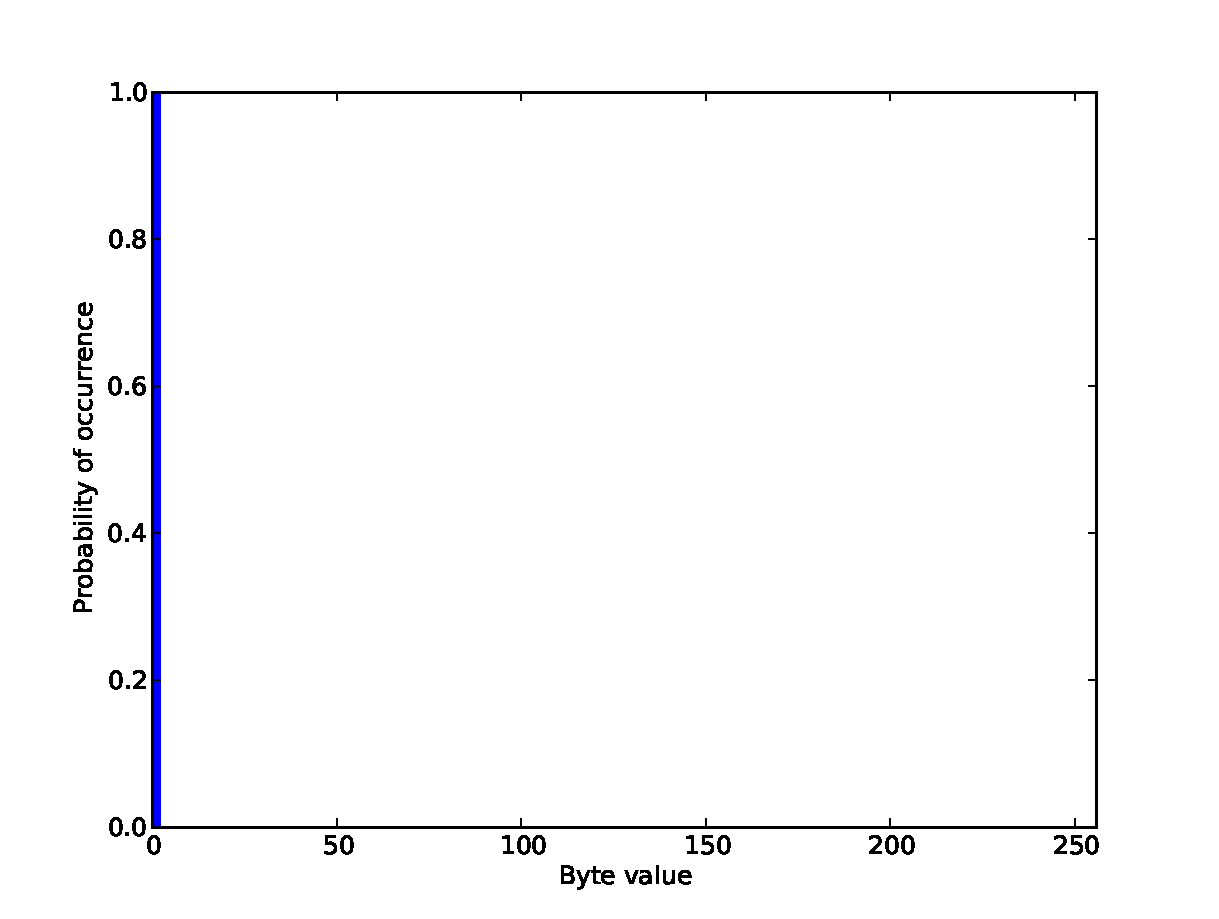
\includegraphics[width=0.8\textwidth]{const_one}
    \captionsetup{width=0.8\textwidth}
    \caption{Byte value distribution of the 6th byte in the DNS header. This
        byte is the least significant byte of the two-byte query count field.
        In our dump its value is constantly one.}
    \label{fig:const_one}
\end{figure}

We define a constant field as a field that only assumes a single value in all
the messages in the current scope. By looking at the byte value probability
distributions, we classify an offset $i$ as constant if $P_{i,v} = 1$ holds for
some $v$, $0 \le v \le 255$. $P_{i,v}$ is an element in the probability
matrix $P$ which is defined in section~\ref{sec:init_clust}.

Constant fields may be interpreted as one of the following:
\begin{itemize}
    \item A true protocol constant. These are fields that are defined to be
        constant in the protocol specification. An example of such a field is
        the protocol field in SMB, which is a four-byte constant field with
        the value \verb+0xff534d42+.
    \item A reserved field. Reserved fields are specified in case there is need
        for future additional information in a fixed-sized header. Reserved
        fields are commonly set to zero.
    \item A field which is constant in the current scope. For example, if a dump
        only contains a single connection, then a session ID field may be
        interpreted as a constant. 
\end{itemize}

\subsection{Flag fields}
\begin{figure}[h]
    \centering
    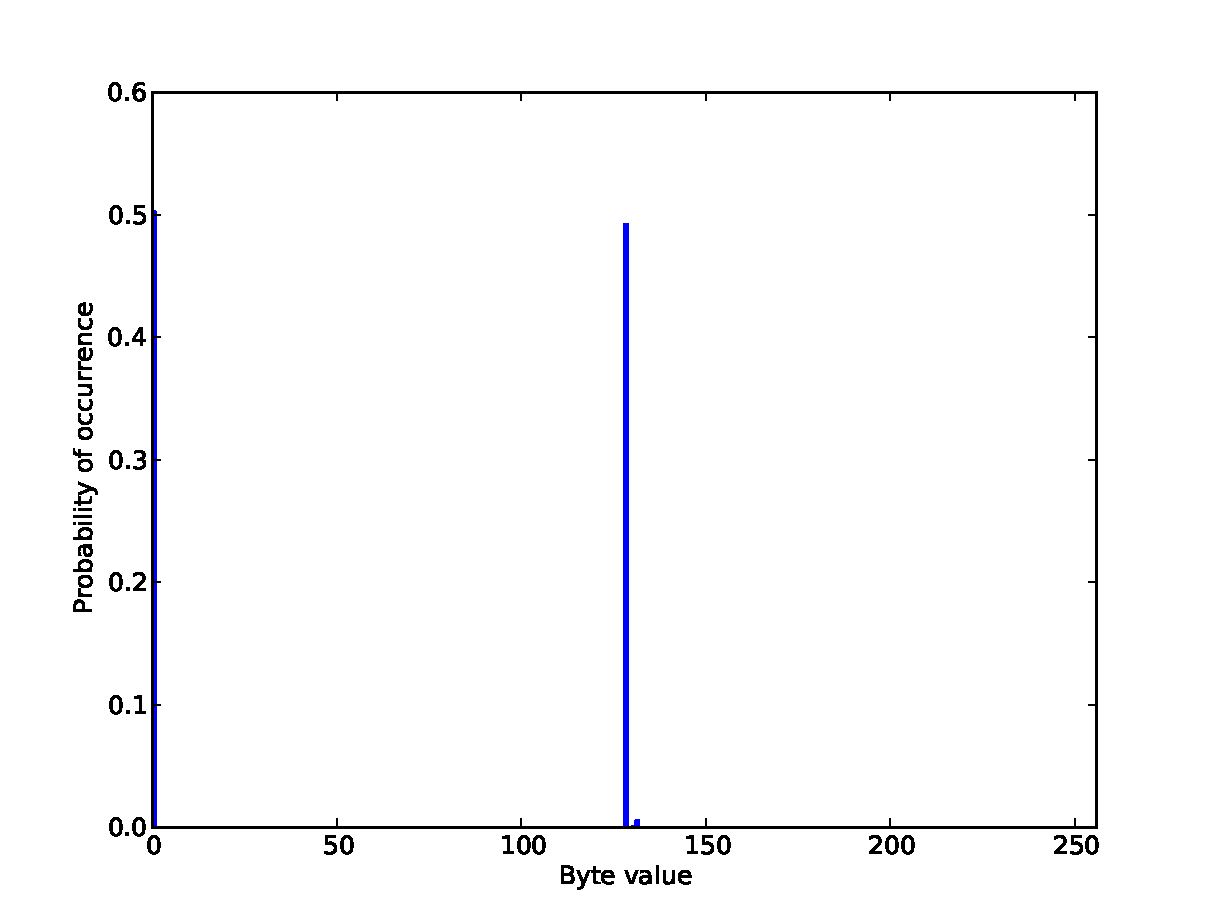
\includegraphics[width=0.8\textwidth]{flag}
    \captionsetup{width=0.8\textwidth}
    \caption{Byte value distribution for the 3rd byte in the DNS header.
    From this byte it may be determined if the message is a query or a
    response.}
    \label{fig:flag}
\end{figure}

A flag field is a field that defines some property of a message. Typically,
it assumes a very limited number of values and may be used for representing
a message type, an error code, a status code and so on.

Flag fields may be interpreted as real numbers where each number represents a numbered entity, such as a
type identifier. It may also represent a set of binary values where each bit
is a flag itself, and is interpreted using a bitmask. An example of such a
field is the DNS flags field. The flag field in DNS is two bytes long, where
the first bit of the field indicates if it is a query (0) or response (1).

The first byte of the DNS flag field is depicted in figure~\ref{fig:flag}.
The amount of queries and responses are relatively equally distributed. The
bar at byte value 0 = \underline{0}0000000 represent the queries. The bar at
byte value 128 = \underline{1}0000000 represent the responses.

When classifying flag fields, we constrain the amount of values that a
certain byte may assume. We classify a field as a flag if the total amount
of values the field takes is greater than one single value and less than
some upper bound.

\subsection{Uniform fields}
\begin{figure}[h]
    \centering
    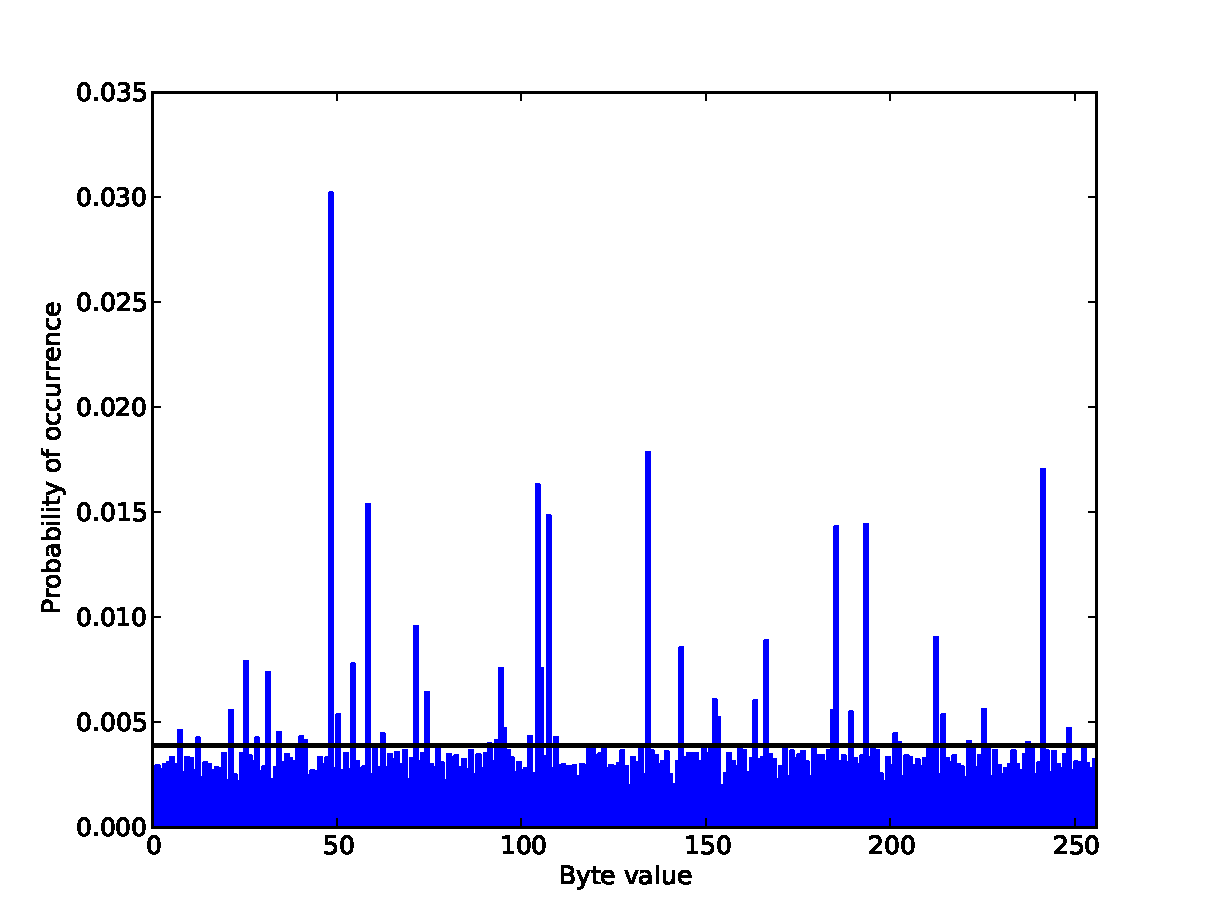
\includegraphics[width=0.8\textwidth]{uniform}
    \captionsetup{width=0.8\textwidth}
    \caption{Byte value distribution for the first byte of the DNS header.
        This byte is the first of a two-byte ID field.}
    \label{fig:uniform}
\end{figure}

A pattern we observed while inspecting the byte value distribution for
various fields was that some fields were uniformly distributed. The real
types of these fields are normally some randomly generated value, such as
a generated session identifier or a nonce.

When classifying fields as uniform, we compare the distribution of the byte
values to the uniform probability distribution for each byte. If we assume the
observed byte value is a random variable $X$ and the expected value the scalar
$x$ then the uniform probability distribution for a byte is

\[
    Pr[X = x] = \left\{
        \begin{array}{l l}
            \frac{1}{256} & \quad 0 \le x \le 255 \\
            0 & \quad \text{otherwise}
        \end{array}
    \right.
\]

If the sum of the deviations from this distribution is below a certain
threshold then the byte is classified as being uniform. If all bytes are
classified as uniform then the field is classified as uniform as well.

In figure~\ref{fig:uniform} the value distribution for the first byte of the
DNS header is displayed. This byte is the first byte of a two-byte identifier.
This ID is generated by the client and used by the DNS server in order to
identify to which query it issues a response. The black line represents the
uniform distribution; a horizontal line at $\frac{1}{256}$.

\subsection{Number fields}

\begin{figure}[h]
    \centering
    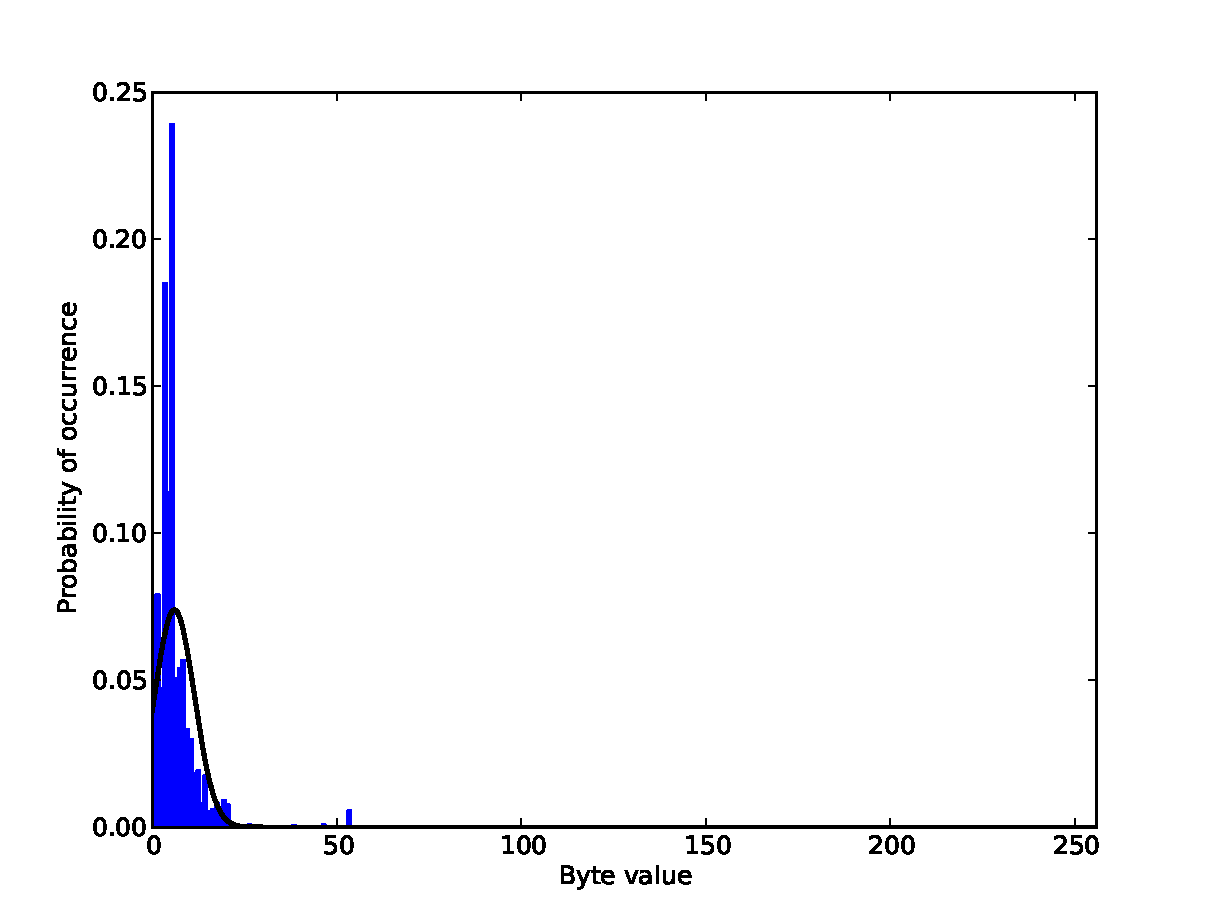
\includegraphics[width=0.8\textwidth]{number}
    \captionsetup{width=0.8\textwidth}
    \caption{A fitted normal distribution to the distribution of values of the
    13th byte in DNS.}
    \label{fig:number}
\end{figure}

While every field in a binary protocol actually contains numbers, some exhibit
a more natural distribution of these numbers than others. We define number
fields as those that can be closely fitted to a normal distribution with
constraints on the standard deviation. We set these constraints so that the
distribution will not collide with our definitions for constant or uniform
fields. This captures the behavior of a random variable $X$ with mean $\mu$ and
standard deviation $\sigma$. Typically, values that represent a count behave
this way, e.g. the QDCOUNT or ANCOUNT fields of the DNS protocols that refer to
how many questions or answers respectively the message contains. This behavior
can also been seen in length fields as they represent a byte count. An example
of such a byte count can be seen in figure~\ref{fig:number}.

\subsection{Incremental fields}
Some protocols contain fields where the value increases for each message in the
scope. It can be a sequence number for each packet or a timestamp of when a
certain action was performed. We define these as incremental fields. These can
be identified by looking at all the messages within a scope and counting how
many of them contain a value that is greater than the previous encountered
value. We then compare this count to the total number of messages in the scope
and if it is above a certain threshold we accept it as being incremental. The
threshold value is used to allow for some amount of wrap-around of the values
in the field.

\subsection{Length fields}

\begin{figure}[h]
    \centering
    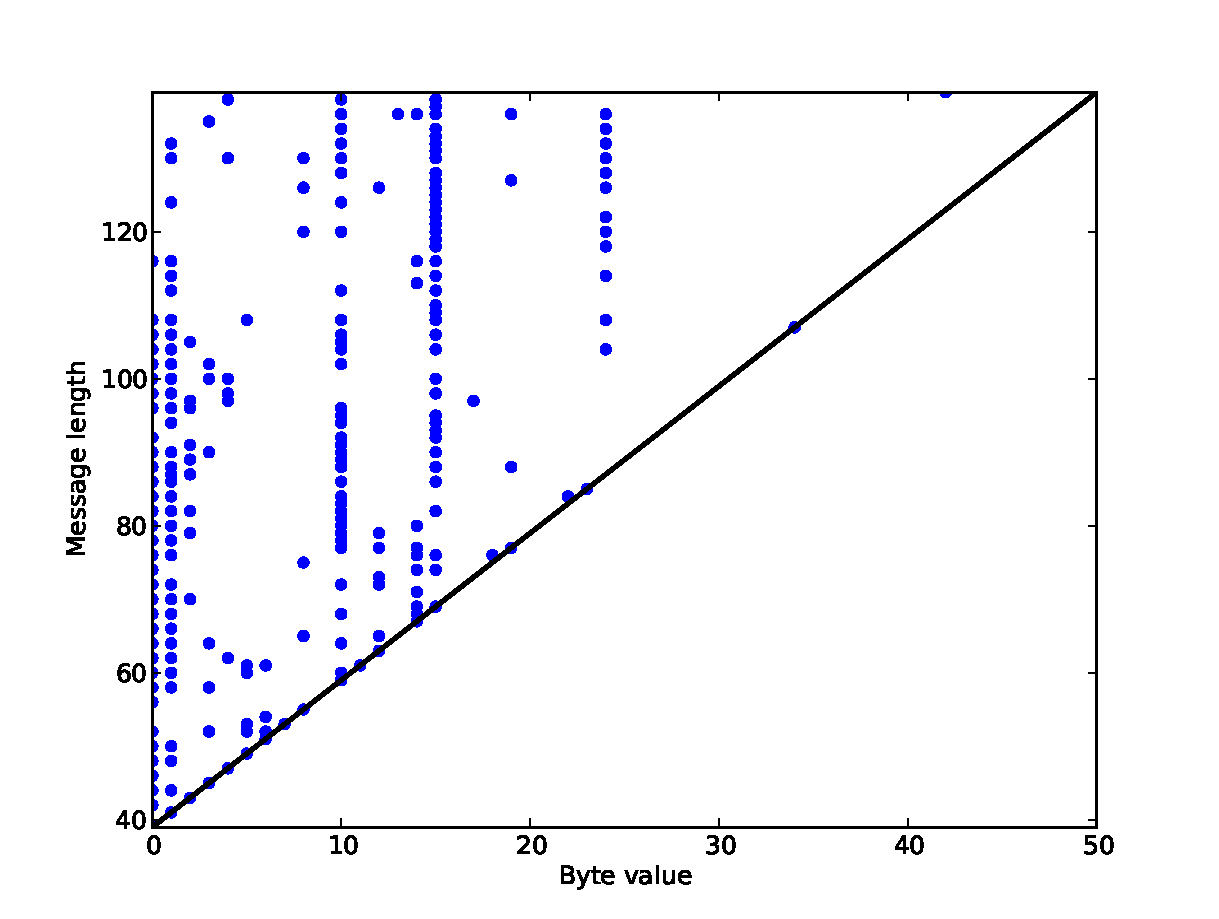
\includegraphics[width=0.8\textwidth]{length}
    \captionsetup{width=0.8\textwidth}
    \caption{RANSAC fit of the WC field in the SMB protocol. The resulting
    parameters are $\alpha = 39$ and $\beta = 2$.}
    \label{fig:length}
\end{figure}

Length fields require the most analysis to identify but also gives a very
confident estimation because of the depth of the analysis. As mentioned in
section~\ref{sec:simplifications}, length fields relate to how long a part of
the message is. This part can be the entire message, the part following the
header or just the next field. For a single message all these types of length
fields can be found, as long as there is only one variable length part in the
message. For the first case the length of the message will be a multiple of the
numerical value in the field. Likewise, in the two last cases, the length will
be a multiple of the numerical value in the field plus an offset equal to the
length of the parts not covered by the field.

Unfortunately, if a message contains multiple parts of variable length the
problem becomes more difficult and cannot be solved by looking at individual
messages anymore. There is however a better way to approach this problem. We
have already seen that the value of the length field multiplied by some scalar
plus an offset (which may be zero) is equal to the length of the message. If
$x$ is the value of the field, $y$ is the length of the message, $\alpha$ is the
offset and $\beta$ is the multiple then this can be written as

\[
    y = \alpha + \beta x
    \label{eq:linlength}
\]

which means that this can be modeled with a linear model. We can then attempt
to solve this with simple linear regression for several messages at once. If
the samples are diverse enough there should be a linear relationship between
the minimum size of all messages with a specific field value and the value
itself. This represents the case of the other variable fields being minimized.
The samples that are not of minimal size for the specific field value will then
be seen as noise. Because of this noise, which normally is the dominant part of
all samples, we need a robust method for fitting our linear model. We therefore
use the RANSAC method as described in section~\ref{sec:ransac} for this
purpose. A real world example of this for the SMB protocol can be seen in
figure~\ref{fig:length}.

One added advantage of using the RANSAC method is that it also handles other
situations where noise appears. This can be if the protocol handles its own
fragmentation or some other form of imperfect parsing that affects the length
of the messages.

\section{Protocol state inference}
Many protocols may be described using a state diagram. Some handshake phase
between the peers is common when a conversation is initialized. There might
also be some teardown phase, and phases for transmitting data etc.
Inferring the states of the protocol is an important task when trying to
figure out the semantics of the protocol. Modelling the protocol states as
a state diagram provides a readable representation of the inner workings
of the protocol, and might simplify the analysis of the fields of the
different message types.

When a reasonable partitioning into types has been achieved, finding the
protocol state diagram is trivial. We simply partition the set of messages
into connections, where connections are tuples of client and server sockets.
From each connection, we define each message in the connection as a change
of state. Each state has a set of probabilities for transitioning to
all other states we've defined. The cumulative sum of these probabilities 
sums up to 1. 

We represent the states as two $n \times n$-matrices, $C$ and  $S$, where 
$n$ is the number of types, which will be the same as the number of states.
Each entry $C_{i,j}$ or $S_{i,j}$ in the matrix defines the numer of times
we observe a transition by the client or server from state $i$ to state $j$.
We define the client as the peer initiating the connection. Once we have our
two matrices, we may calculate the probabilities for the state transitions by
dividing the total number of transitions between two states with the total
number of messages.

A state diagram of all protocol states and transitions may not always be
feasible. Some protocols does not follow the state model which we're 
trying to model with our approach. They may allow some message types to
be sent from all states, and may only be represented with a state diagram
during some phases such as the handshake phase. We handle this problem by
allowing the user to define the depth for which the analysis is performed.
If depth is set to 5, we only analyse which states the protocol may be in
after five transitions. From this restricted state diagram a handshake
procedure will be much more readable.

% Get figure for SMB as well.

In figure~\ref{fig:dnsstate} the state diagram generated from a DNS stream
capture with $MaxNumTypes = 3$ is shown. State 0 represents queries and state 1
represent responses. Blue edges represent messages sent by the client. Red
edges represent messages sent by the client.

Figure~\ref{fig:smbstate} shows the state diagram fom SMB with a depth of
five transitions. This shows the handshake used by the protocol.
Table~\ref{tbl:smb} below lists the true types of the messages in a
left-to-right order with respect to the state diagram.

\begin{figure}
    \centering
    \begin{tabular}{ | l | l |}
        \hline
        \textbf{State}&\textbf{Type}\\ \hline
        37          & Negotiate Protocol Request    \\ \hline
        15          & Negotiate Protocol Response   \\ \hline
        75          & Session Setup AndX Request    \\ \hline
        48          & Session Setup AndX Response   \\ \hline
        14          & Logoff AndX Request           \\ \hline
        50          & Tree Connect AndX Request     \\ \hline
        20          & NT Create AndX Request        \\ \hline
        24          & Delete Request                \\ \hline
    \end{tabular}
    \caption{SMB states.}
    \label{tbl:smb}
\end{figure}

\begin{figure}[h]
    \centering
    \begin{subfigure}[b]{0.48\textwidth}
        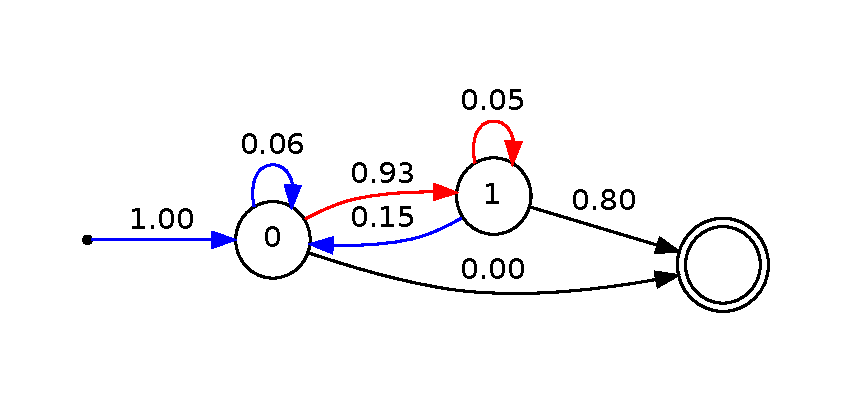
\includegraphics[width=\textwidth]{dnsstate}
        \caption{State diagram for the DNS protocol.}
        \label{fig:dnsstate}
    \end{subfigure}
    \quad
    \begin{subfigure}[b]{0.48\textwidth}
        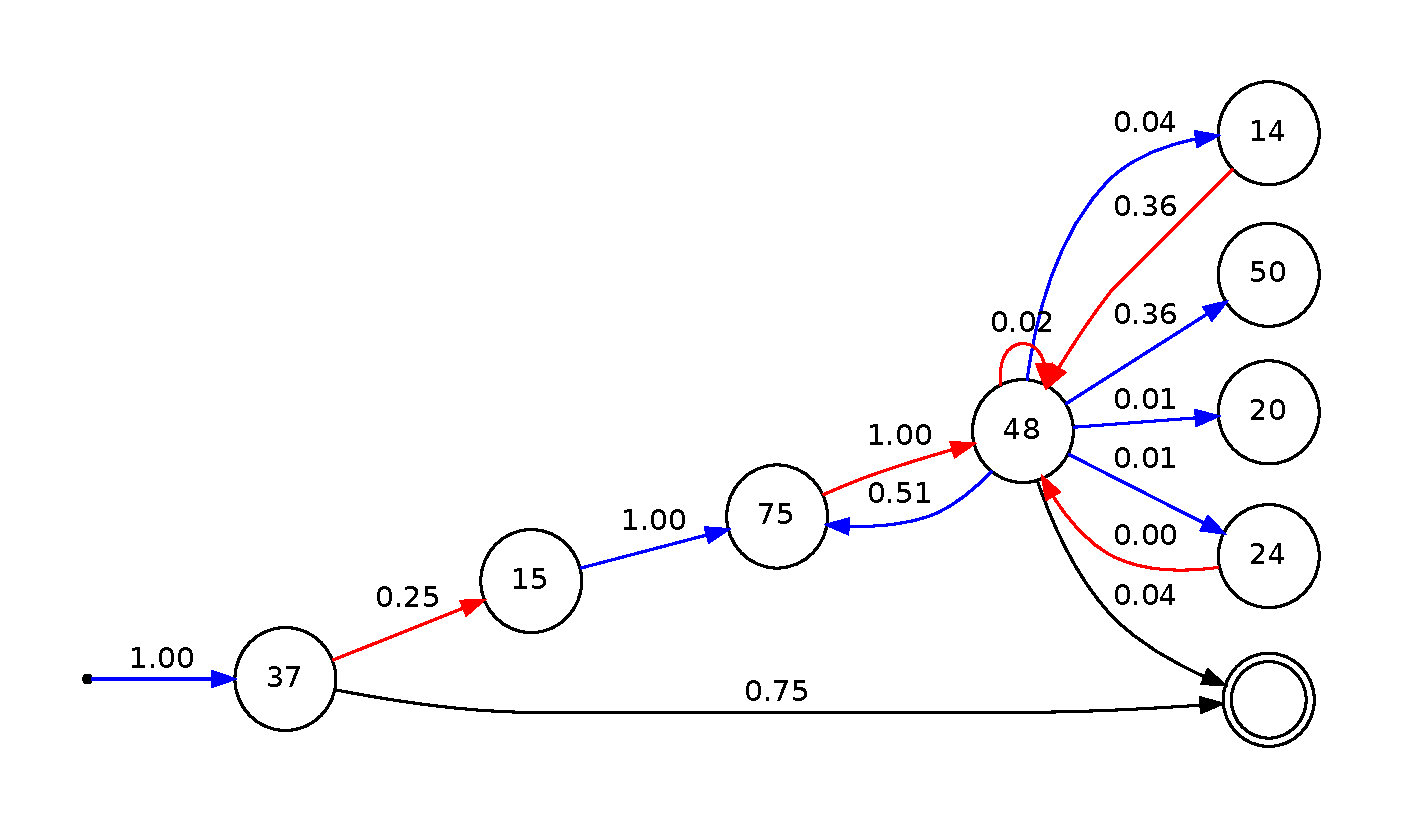
\includegraphics[width=\textwidth]{smbstate}
        \caption{State diagram for the SMB protocol}
        \label{fig:smbstate}
    \end{subfigure}
    \caption{State diagrams generated by our state inference. The left-most
        dot represents the state before any communication has begun. The
        right-most double-circle represents the terminal state.}
    \label{fig:states}
\end{figure}

\chapter{Results}

\section{Data sets}
Provide information about the data used to produce the results.

% SMB
% SMB Command (byte 8), response/request flag (byte 13, bit 0)
% All things with SMB is done on filtered data!

% DNS
% QR OPCODE AA RCODE

% TFTP
% OPCODE (byte 0-1)

% RTP
% Payload Type (byte 1, bit 1-7)

% DHCP
% Message type (byte 0), DHCP Message Type (byte 242)

\begin{figure}
    \centering
    \begin{tabular}{| l | r | r | r |}
        \hline
        \textbf{Protocol}&\textbf{\# Messages}&\textbf{\# Connections}&\textbf{\# Types}\\ \hline
        DNS         & 30628         & 10935         & 6         \\ \hline
        SMB         & 27906         & 212           & 93        \\ \hline
        TFTP        & 6492          & 6             & 3         \\ \hline
        RTP         & 20179         & 5             & 1         \\ \hline
        DHCP        & 13014         & 376           & 11        \\ \hline
    \end{tabular}
    \caption{Datasets.}
\end{figure}

\section{Clustering performance}
Display the results of applying our method to different data sets.
% Metrics: homogenity, completeness, V-Measure
% Improvement over dump size; all metrics
%   Before type distinguisher clustering
%   After type distringuisher clustering

\begin{figure}
    \centering
    \begin{tabular}{| l | r | r | r |}
        \hline
        \textbf{Protocol}&\textbf{minSamples}&\textbf{maxNumTypes}&\textbf{Limit} \\ \hline
        DNS & 200 & 10 & 200 \\ \hline
        SMB & 50 & 100 & 200 \\ \hline
        TFTP & 50 & 10 & 200 \\ \hline
        RTP & 200 & 10 & 200 \\ \hline
        DHCP & 50 & 20 & 400 \\ \hline
    \end{tabular}
    \caption{Clustering parameters.}
\end{figure}

\begin{figure}
    \centering
    \begin{tabular}{| l | r | r | r | r | r |}
        \hline
        \textbf{Protocol}&\textbf{Completeness}&\textbf{Homogenity}&\textbf{V-measure} \\ \hline
        DNS & 0.1982 & 0.9550 & 0.3282 \\ \hline
        SMB & 0.8480 & 0.8632 & 0.8555 \\ \hline
        TFTP & 0.3015 & 0.9449 & 0.4571 \\ \hline
        RTP & 0.0000 & 1.0000 & 0.0000 \\ \hline
        DHCP & 0.3492 & 0.1224 & 0.1813 \\ \hline
    \end{tabular}
    \caption{Before type distinguisher clustering.}
\end{figure}

\begin{figure}
    \centering
    \begin{tabular}{| l | r | r | r | r | r |}
        \hline
        \textbf{Protocol}&\textbf{Completeness}&\textbf{Homogenity}&\textbf{V-measure} \\ \hline
        DNS & 0.9534 & 0.9999 & 0.9761 \\ \hline
        SMB & 0.9914 & 0.9880 & 0.9897 \\ \hline
        TFTP & 1.0000 & 1.000 & 1.000 \\ \hline
        RTP & 0.0000 & 1.0000 & 0.0000 \\ \hline
        DHCP & 1.0000 & 0.4428 & 0.6138 \\ \hline
    \end{tabular}
    \caption{After type distinguisher clustering.}
\end{figure}

\section{Field inference performance}
% Compare each byte to annotation. Measure is the percentage of correctly
% inferred bytes. Perform for both cluster and header (two different 
% subsections?)
%
% Field boundaries: Check false positives/negatives

\chapter{Discussion}

\section{Conclusions}
Draw conclusions about our method and compare it to the related methods.

Is sequence alignment necessary? We could iteratively find length fields to get
perfect alignments. Delimiters might be a problem

\section{Limitations}
Give a short introduction to the different limitations of our method.

Mention that the scoring matrix could be improved to use a normal distribution
for scoring numerical differences.

Mention the problem with our restricted version of multiple sequence alignment
that it the longest message could optimally need gap insertion as well.

\subsection{Textual protocols}
Explain why our method is not applicable to textual protocols.

\subsection{Variable number of fields}
Explain the problem with protocols that contain a variable number of fields and
why our method does not accommodate for them. (Because we based our definition
of protocols on a fixed number of fields?)

\subsection{Non-aligned data}
Explain why we only try to find aligned fields and the problem with complexity
if we were to relax this requirement.

\subsection{Bit precision}
Talk a little bit about how some protocols do not use entire bytes as the sizes
of their fields and that we will not find exact boundaries for them.

\section{Future work}
Mention the ideas that has come up during the thesis work that we have not had
time to investigate further.

\subsection{Correspondence analysis}
Explain how correspondence analysis could give a better result than PCA.

\subsection{Timestamp identification}
Explain how timestamps could potentially be identified from their distinguished
byte distribution pattern.

\bibliographystyle{plainnat}
\bibliography{thesis}

\end{document}

